Una vez que obtenemos para cada algoritmos la mejor combinación de resultados, se ejecutan los modelos calculados con el conjunto de test y de entrenamiento inicial. De esta forma se pretende estimar el sobreajuste, ``overfitting'', del modelo. 

\section{Concepto de sobreajuste}
El sobreajuste u ``overfitting'' se produce cuando un modelo cuando obtiene muy buenos resultados bien con los datos de entrenamiento, pero su precisión es notablemente más baja con el conjunto de test. Esto se produce porque el modelo se ha adaptado a los valores del conjunto de entrenamiento y no es capaz de generalizar para datos que no ha procesado. En la imagen \ref{figure:sobreajuste} podemos observar gráficamente en que consiste este problema.

\begin{figure}[H]
\centering
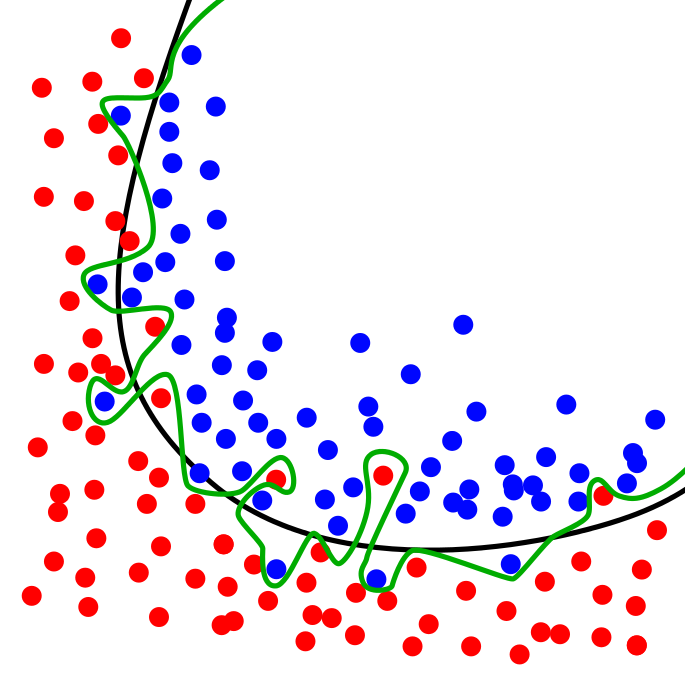
\includegraphics[width=0.3\textwidth]{figs/Overfitting.png}
\caption{Ejemplo de sobreajuste, línea verde \cite{SobreajusteLibre}}
\label{figure:sobreajuste}
\end{figure}

Este sobreajuste está directamente relacionado con la complejidad del modelo, cuanto más complejo sea más tendencia tendrá a sobreajustarse. Aparte, si el conjunto de datos del que disponemos es reducido, como en nuestro caso, este problema de sobreajuste estará muy presente.

\section{Resumen de los resultados}

En la tabla \ref{table:resultados} podemos ver para cada algoritmo los resultados obtenidos cuando se ejecuta la mejor configuración obtenida en los pasos anteriores. Entre los resultados se distinguen los valores para el conjunto de entrenamiento y para el conjunto de test. De esta forma controlamos el sobreajuste anteriormente descrito.


\begin{table}[H]
\centering
\begin{tabular}{c|c|c|c|c|}
\cline{2-5}
                                        & \multicolumn{2}{c|}{\textbf{Todas las matrices}} & \multicolumn{2}{c|}{\textbf{Matrices de DTI}} \\ \cline{2-5} 
                                        & \textbf{Test}          & \textbf{Train}          & \textbf{Test}         & \textbf{Train}        \\ \hline
\multicolumn{1}{|c|}{\textbf{Logistic Regression}} & 72.73\%                & 67.69\%                 & 78.57\%               & 84.42\%               \\ \hline
\multicolumn{1}{|c|}{\textbf{Support Vector Machine}}      & 72.73\%                & 100\%                   & 78.72\%               & 100\%                 \\ \hline
\multicolumn{1}{|c|}{\textbf{Gaussian Naive Bayes}}    & 60.61\%                & 70.77\%                 & 78.72\%               & 86.02\%               \\ \hline
\multicolumn{1}{|c|}{\textbf{Random Forest Classifier}}   & 72.73\%                & 96.92\%                 & 74.47                 & 93.55\%               \\ \hline
\multicolumn{1}{|c|}{\textbf{Artificial Neural Network}}      & 65.00\%                & 70.51\%                 & 82.14                 & 82.14\%               \\ \hline
\end{tabular}
\caption{Tabla resumen de los resultados de los experimentos por algoritmo}
\label{table:resultados}

\end{table}

\section{Precisión,  exhaustividad y  medida-F1}

En las imágenes 
\ref{figure:logall}, 
\ref{figure:logdti}, 
\ref{figure:svmall}, 
\ref{figure:svmdti}, 
\ref{figure:bayesall}, 
\ref{figure:bayesdti},
\ref{figure:forestall},
\ref{figure:forestdit},
\ref{figure:annall} y
\ref{figure:anndti},
 extraídas de los resultados podemos ver para cada algorimos los resultados de las dos ejecuciones: considerando todas las matrices o solamente las \gls{dti}. En cada una se puede ver para cada clase (1, 0) los valores de precisión (precision), exhaustividad (recall) y la medida-F1 (f1-score) para cada uno de las ejecuciones. Estas tres medidas están relacionadas con los errores de tipo I y tipo II. 

\begin{figure}[H]
\centering
\fbox{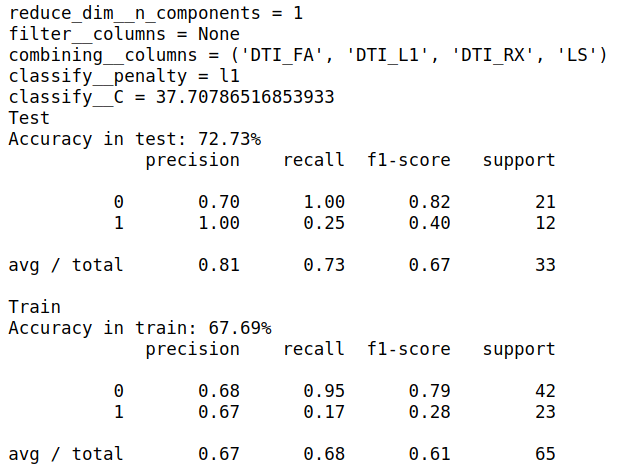
\includegraphics[width=0.5\textwidth]{figs/resultados/log_all.png}}
\caption{Resultado ejecución algoritmo Logistic Regression. Considerando todas las matrices.}
\label{figure:logall}
\end{figure}

\begin{figure}[H]
\centering
\fbox{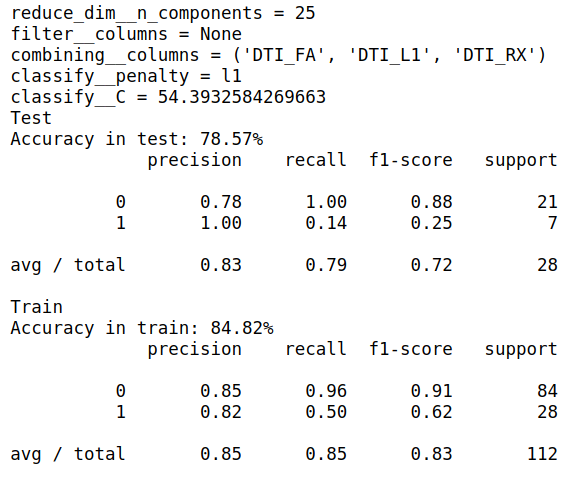
\includegraphics[width=0.5\textwidth]{figs/resultados/log_dti.png}}
\caption{Resultado ejecución algoritmo Logistic Regression. Considerando sólo matrices \gls{dti}.}
\label{figure:logdti}
\end{figure}

\begin{figure}[H]
\centering
\fbox{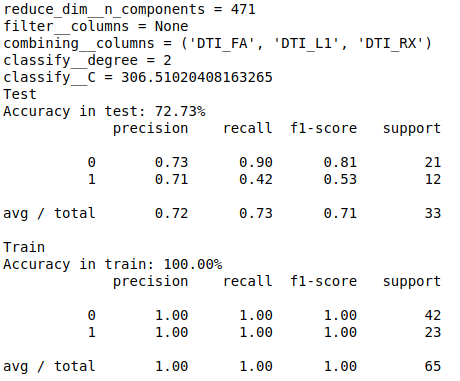
\includegraphics[width=0.5\textwidth]{figs/resultados/svm_all.png}}
\caption{Resultado ejecución algoritmo Support Vector Machine. Considerando todas las matrices.}
\label{figure:svmall}
\end{figure}

\begin{figure}[H]
\centering
\fbox{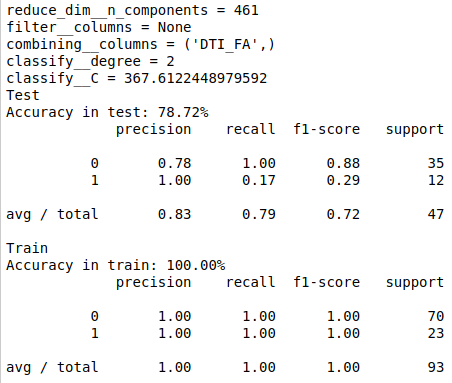
\includegraphics[width=0.5\textwidth]{figs/resultados/svm_dti.png}}
\caption{Resultado ejecución algoritmo Support Vector Machine. Considerando sólo matrices \gls{dti}.}
\label{figure:svmdti}
\end{figure}

\begin{figure}[H]
\centering
\fbox{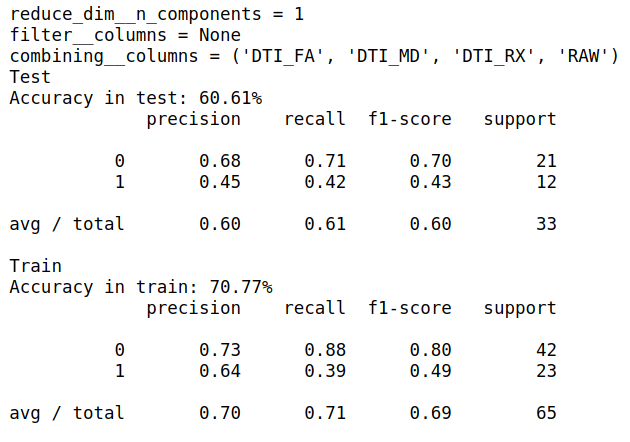
\includegraphics[width=0.5\textwidth]{figs/resultados/bayes_all.png}}
\caption{Resultado ejecución algoritmo Gaussian Naive Bayes. Considerando todas las matrices.}
\label{figure:bayesall}
\end{figure}

\begin{figure}[H]
\centering
\fbox{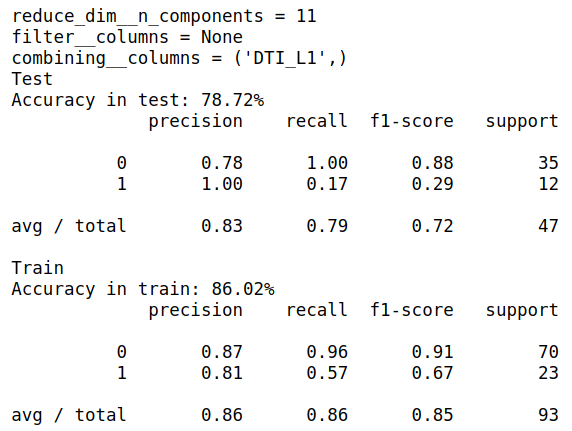
\includegraphics[width=0.5\textwidth]{figs/resultados/bayes_dti.png}}
\caption{Resultado ejecución algoritmo Gaussian Naive Bayes. Considerando sólo matrices \gls{dti}.}
\label{figure:bayesdti}
\end{figure}

\begin{figure}[H]
\centering
\fbox{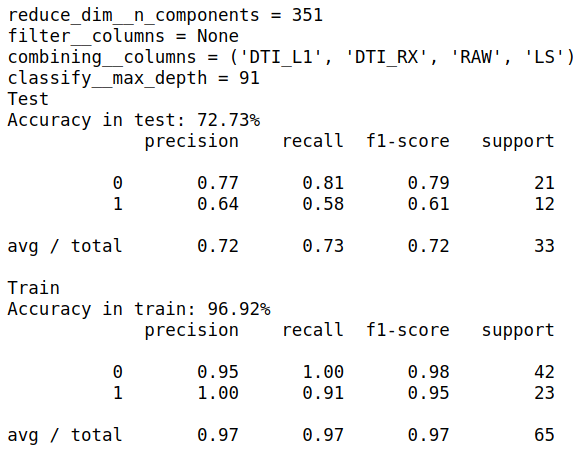
\includegraphics[width=0.5\textwidth]{figs/resultados/forest_all.png}}
\caption{Resultado ejecución algoritmo Random Forest Classifier. Considerando todas las matrices.}
\label{figure:forestall}
\end{figure}

\begin{figure}[H]
\centering
\fbox{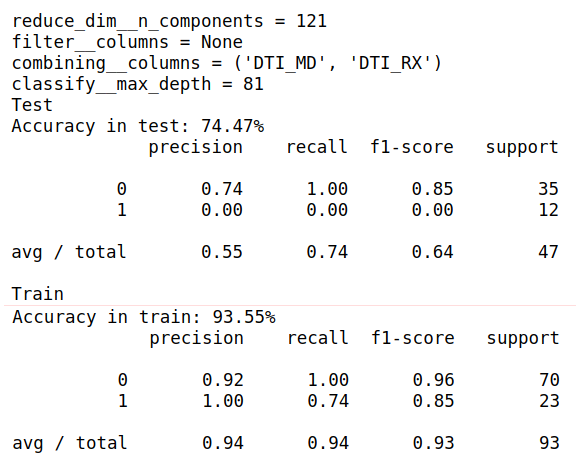
\includegraphics[width=0.5\textwidth]{figs/resultados/forest_dti.png}}
\caption{Resultado ejecución algoritmo Random Forest Classifier. Considerando sólo matrices \gls{dti}.}
\label{figure:forestdit}

\end{figure}
\begin{figure}[H]
\centering
\fbox{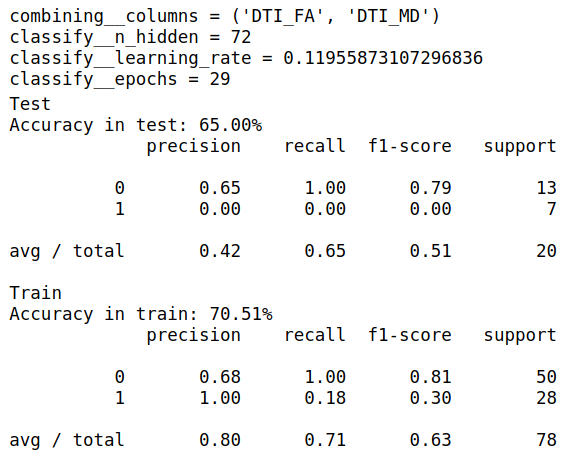
\includegraphics[width=0.5\textwidth]{figs/resultados/ann_all.png}}
\caption{Resultado ejecución algoritmo Artificial Neural Network. Considerando todas las matrices.}
\label{figure:annall}
\end{figure}

\begin{figure}[H]
\centering
\fbox{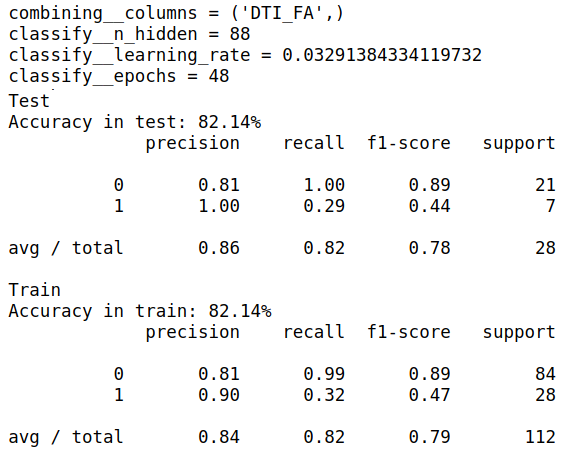
\includegraphics[width=0.5\textwidth]{figs/resultados/ann_dti.png}}
\caption{Resultado ejecución algoritmo Artificial Neural Network. Considerando sólo matrices \gls{dti}.}
\label{figure:anndti}
\end{figure}

La precisión es la habilidad del clasificador etiquetar correctamente los valores dentro de su grupo. La exhaustividad en cambio es la habilidad para acertar con las etiquetas en todo el conjunto. Por ejemplo, si disponemos de 10 ejemplares de donde 3 son del tipo A y 7 son del tipo B. A través de nuestro modelo obtenemos 5 elementos del tipo A pero sólo 2 han sido correctamente etiquetados, entonces nuestra precisión sería 2/3 y la exhaustividad 2/10. La medida-F1 engloba las otras dos siendo un valor único ponderado de la precisión y la exhaustividad. Su valor se calcula con la siguiente fórmula: 

$$F_1 = \frac{2}{\tfrac{1}{\mathrm{recall}} + \tfrac{1}{\mathrm{precision}}} = 2 \cdot \frac{\mathrm{precision} \cdot \mathrm{recall}}{\mathrm{precision} + \mathrm{recall}}$$

Aunque en este trabajo nos hemos centrado en una mejor ``accuracy'' pero igualmente, dependiendo de la finalidad de los experimentos se pueden ajustar para que la selección de los parámetros de la configuración tuviese como meta alguno de éstos.
